\section{Introduction to ZX-Calculus}

As stated in the previous section, the ZX-Calculus represents the
$\mathbf{FDHilb}$ category. This means that the objects of our category are finite dimensional Hilbert spaces and the morphisms are linear maps between those Hilbert spaces. We are going to  represent the morphisims as $\textit{Spiders}$. So in total the whole classical quantum circuit is represented as a graph of morphism/spiders. In this representation it is very easy to to apply simplification rules to the circuit.

\subsection{Spiders}

Spiders are the $\textit{atoms}$ of a ZX-Diagram. They represent the decomposition of quantum gates into even smaller and more fundamental operations. Some important decompositions are shown in figure \ref{fig:spiders-gate-representation}.

Spiders can have an arbitrary number of incoming and outgoing edges and appear in two flavors: $\textit{Z-Spiders}$ and $\textit{X-Spiders}$. This distinction is shown visually using the green and red color respectively when drawing the spiders.
Additionally spiders may carry a phase value $\alpha \in [0, 2\pi)$. Which can be ommited if it is zero.

In figure \ref{fig:spiders-visual} the spiders are shown visually. The first spider is a $\textit{Z-Spider}$ and the second one is an $\textit{X-Spider}$. Both have $n$ incoming and $m$ outgoing edges and carry a phase value $\alpha$.

\begin{figure}[h]
    \centering
    \begin{ZX}
        \leftManyDots{n}  \zxZ{\alpha} \rightManyDots{m}
    \end{ZX}
    \begin{ZX}
        \leftManyDots{n}  \zxX{\alpha} \rightManyDots{m}
    \end{ZX}
    \caption{Fundamental spiders with $n$ incoming and $m$ outgoing edges}
    \label{fig:spiders-visual}
\end{figure}


It is important to remember that each spider represents a morphism in the $\mathbf{FDHilb}$ category. This means that each spider represents a linear map from the incoming $n$ to the outgoing $m$ qubits. Those linear maps are shown in figure \ref{fig:individual-spiders-linear-maps}.

\begin{figure}[h]
    \begin{align*}
        \begin{ZX}
            \leftManyDots{n}  \zxZ{\alpha} \rightManyDots{m}
        \end{ZX}
        :=                                               & |\underbrace{0\dots 0}_{m}\rangle \langle \underbrace{0\dots0}_{n}| + e^{i\alpha}|\underbrace{1\dots1}_{m}\rangle \langle \underbrace{1\dots1}_{n}|
        \\
        =                                                & \begin{pmatrix}
                                                               1      & 0      & \dots  & 0           \\
                                                               0      & 0      & \dots  & 0           \\
                                                               \vdots & \vdots & \ddots & \vdots      \\
                                                               0      & 0      & \dots  & e^{i\alpha} \\
                                                           \end{pmatrix}
        \\
        \begin{ZX}
            \leftManyDots{n}  \zxX{\alpha} \rightManyDots{m}
        \end{ZX} := & |\underbrace{+ \dots +}_{m}\rangle \langle \underbrace{- \dots -}_{n}| + e^{i\alpha}|\underbrace{- \dots -}_{m}\rangle \langle \underbrace{+ \dots +}_{n}|
        \\
    \end{align*}
    \caption{Linear maps represented by individual spiders}
    \label{fig:individual-spiders-linear-maps}
\end{figure}

Note that the linear maps in figure \ref{fig:individual-spiders-linear-maps} do not have to be unitary, nor do they have to square. The dimension of the linear map depends only on the number of incoming and outgoing edges. For example, a spider with $n$ incoming and $m$ outgoing edges represents a linear map in $\mathbb{C}^{2^m \times 2^n}$.


\subsection{Classical Quantum Gates as Spiders}

\begin{figure}
    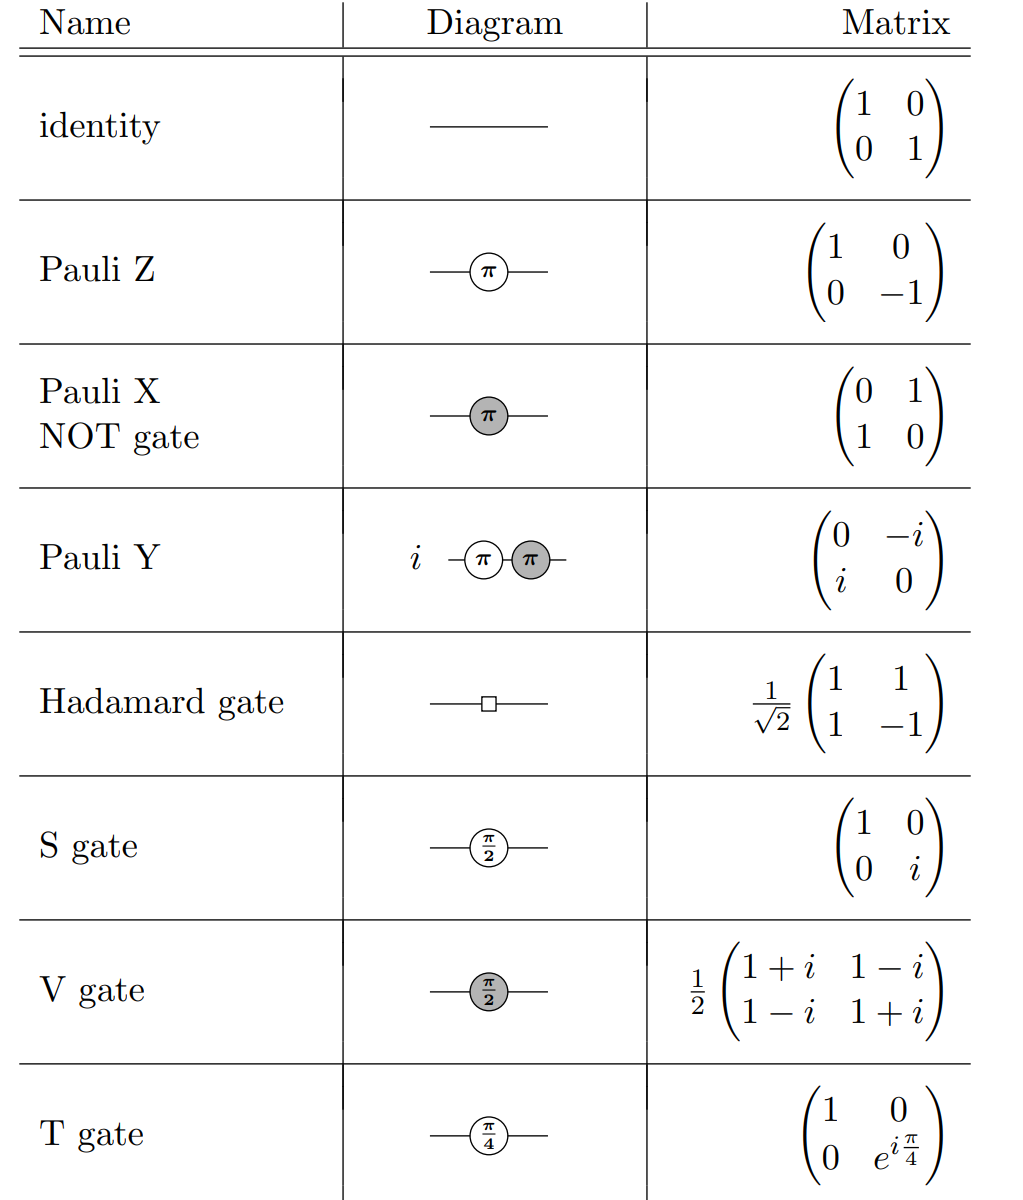
\includegraphics[width=\linewidth]{images/single_spider_unitaries.png}
    \caption{Spiders representing quantum gates
            {\cite{vandewetering2020zxcalculus}[P.87]}}
    \label{fig:spiders-gate-representation}
\end{figure}



By just using the single spiders shown in figure \ref{fig:spiders-visual} we can already represent a lot of quantum gates. The most important ones are shown in figure \ref{fig:spiders-gate-representation}. Note that we are going to ignore the global scalar values of ZX-Diagrams in the following sections, since they are negligible for most cases \cite{equivalence_checking_tum}. Furthermore, when working with unitary circuits, the scalar value can be restored at the end of the calculation as the resulting circuit-matrix is proportional to the unitary matrix \cite{vandewetering2020zxcalculus}.


It is easy to verify that the gates from the figure \ref{fig:spiders-gate-representation} can indeed be represented using just the basic spiders. This boils down just inserting the corresponding spiders into the formulas from figure \ref{fig:individual-spiders-linear-maps} and to compare the resulting matrices with the matrices of the Pauli gates.
These proofs are shown in figures \ref{appendix:pauli-z-gate-as-spider}, \ref{appendix:pauli-x-gate-as-spider} and \ref{appendix:pauli-y-gate-as-spider}.

\subsection{Bigger Circuits}

Using the rules from figure \ref{fig:spiders-gate-representation} we can only represent circuits consisting of a single gate. For bigger circuits we need to combine multiple spiders into a single diagram. This is done by connecting the spiders leg to leg. This means that the outgoing legs of one spider are connected to the incoming legs of another spider.

But before we can work with such circuits we need to define some more rules to calculate the matrix representation of a circuit.

\begin{enumerate}

    \item \textbf{Only Topology Matters}

          The first rule is that we can move spiders around freely, as long as we maintain the correct order of the incoming andoutgoing legs. This rule corresponds to the $\textit{Only Topology Matters}$ mantra of the ZX-Calculus.

    \item \textbf{Parallel Composition}
          The second rule allows to calculate the matrix representation of spiders acting in parallel. We have seen this rule bevore, when we looked at the category representation of the ZX-Calculus (\ref{parallel-composition}). In $\mathbf{FDHilb}$ this rule corresponds to the kroncker product of matrices for the individual spiders.

    \item \textbf{Sequential Composition}
          The third rule allows to calculate the matrix representation of spiders acting in sequence. This rule corresponds to the sequential composition (\ref{sequential-composition}) in the category representation of the ZX-Calculus. In particular it allows to calculate the matrix representation such a circuit by multiplying the matrices of the individual spiders.
\end{enumerate}

\subsection{Example: CNOT Gate}

An example for a circuit consisting of multiple spiders is the classical CNOT gate, which can be represented by the ZX-Diagram shown in figure \ref{fig:cnot-gate-split}.

In order to calculate the matrix representation of this circuit we first need to split the circuit into the individual spiders. The result this process is already shown in figure \ref{fig:cnot-gate-split-4}.

\begin{figure}[h]
    \centering
    \subfloat[\centering CNOT split into 4 Regions\label{fig:cnot-gate-split-4}]{{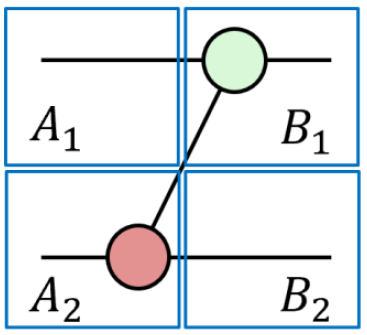
\includegraphics[height=3.5cm]{images/cnot-regions-4.png} }}
    \qquad
    \subfloat[\centering CNOT split into 2 Regions\label{fig:cnot-gate-split-2}]{{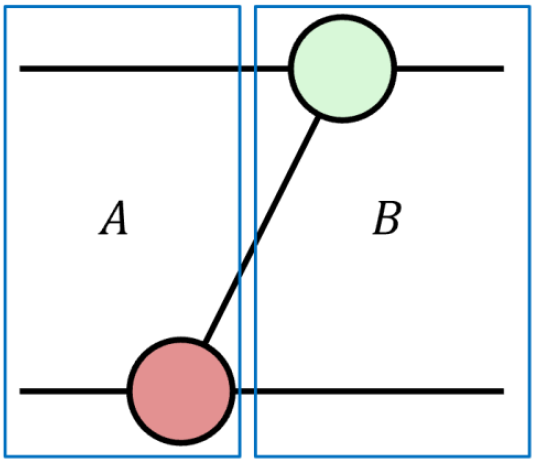
\includegraphics[height=3.5cm]{images/cnot-regions-2.png} }}
    \caption{Splitting the CNOT gate into regions}
    \label{fig:cnot-gate-split}
\end{figure}

Using the rules we just defined we can now calculate the matrix representation of the circuit. We start by applying the $\textit{Parallel Composition}$ rules, to combine sections $A_1$ and $A_2$ into a new section $A$. The same is done for sections $B_1$ and $B_2$ to create section $B$. This reduction results in the ZX-Diagram shown in figure \ref{fig:cnot-gate-split-2}.


The calculation looks as follows:


\begin{align*}
    A & = A_1 \otimes A_2                           \\
      & = id \otimes \text{RedSpider($n=1$, $m=2$)} \\
      & =id    \otimes
    |+\rangle \langle ++| + |-\rangle \langle --|   \\
      & = \begin{pmatrix}
              1 & 0 \\
              0 & 1 \\
          \end{pmatrix}
    \otimes
    \frac{1}{\sqrt{2}}
    \begin{pmatrix}
        1 & 0 \\
        0 & 1 \\
        0 & 1 \\
        1 & 0 \\
    \end{pmatrix}                                  \\
      & = \frac{1}{\sqrt{2}}
    \begin{pmatrix}
        1 & 0 & 0 & 0 \\
        0 & 1 & 0 & 0 \\
        0 & 1 & 0 & 0 \\
        1 & 0 & 0 & 0 \\
        0 & 0 & 1 & 0 \\
        0 & 0 & 0 & 1 \\
        0 & 0 & 0 & 1 \\
        0 & 0 & 1 & 0 \\
    \end{pmatrix}
\end{align*}

\begin{align*}
    B & = B_1 \otimes B_2                             \\
      & = \text{GreenSpider($n=2$, $m=1$)} \otimes id \\
      & =
    \begin{pmatrix}
        1 & 0 & 0 & 1 \\
        0 & 1 & 1 & 0 \\
    \end{pmatrix}
    \otimes
    \begin{pmatrix}
        1 & 0 \\
        0 & 1 \\
    \end{pmatrix}                                    \\
      & = \begin{pmatrix}
              1 & 0 & 0 & 1 & 0 & 0 & 0 & 0 \\
              0 & 1 & 1 & 0 & 0 & 0 & 0 & 0 \\
              0 & 0 & 0 & 0 & 1 & 0 & 0 & 1 \\
              0 & 0 & 0 & 0 & 0 & 1 & 1 & 0 \\
          \end{pmatrix}
\end{align*}


Now we have calculated all Regions from figure \ref{fig:cnot-gate-split-2} and can combine them into a single matrix. For this we apply the $\textit{Sequential Composition}$ rule to combine sections $A$ and $B$ into a new section $R$.

The calculation looks as follows:


\begin{align*}
    R & = A \circ B         \\
      & = B \cdot A         \\
      & =
    \frac{1}{\sqrt{2}}
    \begin{pmatrix}
        1 & 0 & 0 \\
        0 & 1 & 0 \\
        0 & 0 & 1 \\
        0 & 1 & 0 \\
    \end{pmatrix}          \\
      & \propto \text{CNOT}
\end{align*}

The resulting matrix is proportional to the matrix representation of the CNOT gate. This means that the ZX-Diagram \zx{
    \zxNone{} \rar & \zxNone{} \rar  &\zxZ{}\rar  &\\
    \zxNone{} \rar & \zxX{} \rar \ar[ru]  &\rar& \\
} is indeed a valid representation of the CNOT gate.


